\documentclass[11pt,a4paper]{article}

% ====================================================================
% Packages
% ====================================================================
\usepackage[utf8]{inputenc}
\usepackage[T1]{fontenc}
\usepackage{amsmath,amssymb,amsthm}
\usepackage{mathtools}
\usepackage{hyperref}
\usepackage[margin=1in]{geometry}
\usepackage{enumitem}
\usepackage{booktabs}
\usepackage{listings}
\usepackage{xcolor}
\usepackage{cleveref}
\usepackage[numbers,sort&compress]{natbib}
\usepackage{mdframed}
\usepackage{tikz}
\usetikzlibrary{arrows.meta,positioning}
\usepackage{longtable}

% ====================================================================
% Theorem environments
% ====================================================================
\theoremstyle{plain}
\newtheorem{theorem}{Theorem}[section]
\newtheorem{lemma}[theorem]{Lemma}
\newtheorem{proposition}[theorem]{Proposition}
\newtheorem{corollary}[theorem]{Corollary}

\theoremstyle{definition}
\newtheorem{definition}[theorem]{Definition}
\newtheorem{remark}[theorem]{Remark}

% ====================================================================
% Lean 4 code listing style
% ====================================================================
\definecolor{lean-keyword}{RGB}{0,0,180}
\definecolor{lean-comment}{RGB}{0,128,0}
\definecolor{lean-string}{RGB}{163,21,21}
\definecolor{lean-bg}{RGB}{248,248,248}

\lstdefinelanguage{lean4}{
  keywords={theorem,lemma,def,class,instance,import,open,variable,
            noncomputable,section,namespace,end,where,let,have,show,
            intro,obtain,use,exact,rw,simp,apply,by,fun,match,if,
            then,else,do,return,axiom,abbrev,private,attribute,
            suffices,change,congr,ext,constructor,rintro,push_neg,
            linarith,absurd,set_option,omit,in,set,cases,left,right,
            nlinarith,push_cast,positivity,omega,refine,field_simp,
            structure,calc,ring,fun_prop,unfold,induction,deriving,
            inductive,rcases,first,all_goals,trivial,convert},
  sensitive=true,
  morecomment=[l]{--},
  morecomment=[s]{/-}{-/},
  morestring=[b]",
  morestring=[b]',
}

\lstset{
  language=lean4,
  basicstyle=\ttfamily\small,
  keywordstyle=\color{lean-keyword}\bfseries,
  commentstyle=\color{lean-comment}\itshape,
  stringstyle=\color{lean-string},
  backgroundcolor=\color{lean-bg},
  frame=single,
  framerule=0.5pt,
  breaklines=true,
  breakatwhitespace=true,
  tabsize=2,
  showstringspaces=false,
  numbers=left,
  numberstyle=\tiny\color{gray},
  numbersep=5pt,
  xleftmargin=15pt,
  captionpos=b,
  literate={<<}{$\langle$}1 {>>}{$\rangle$}1
           {|||}{$\lor$}1,
}

% ====================================================================
% Macros
% ====================================================================
\newcommand{\NN}{\mathbb{N}}
\newcommand{\RR}{\mathbb{R}}
\newcommand{\ZZ}{\mathbb{Z}}
\newcommand{\LPO}{\ensuremath{\mathrm{LPO}}}
\newcommand{\WLPO}{\ensuremath{\mathrm{WLPO}}}
\newcommand{\LLPO}{\ensuremath{\mathrm{LLPO}}}
\newcommand{\BISH}{\ensuremath{\mathrm{BISH}}}
\newcommand{\BMC}{\ensuremath{\mathrm{BMC}}}
\newcommand{\FT}{\ensuremath{\mathrm{FT}}}
\newcommand{\MP}{\ensuremath{\mathrm{MP}}}
\newcommand{\DC}{\ensuremath{\mathrm{DC}}}
\newcommand{\Lean}{\textsc{Lean~4}}
\newcommand{\Mathlib}{\textsc{Mathlib4}}
\newcommand{\leanok}{\textsf{\small \textcolor{green!70!black}{\checkmark}}}
\newcommand{\leanaxiom}{\textsf{\small \textcolor{orange!80!black}{(axiom)}}}

% ====================================================================
% Title
% ====================================================================
\title{%
  \textbf{What the Ceiling Means:\\
  Constructive Schools, Physical Actualisation,\\
  and the Fine Structure of BISH+LPO}\\[6pt]
  {\normalsize A Lean~4 Formalization (Paper~43)}%
}

\author{
  Paul Chun-Kit Lee\thanks{%
    New York University.
    AI-assisted formalization; see \S\ref{sec:lean} for methodology.} \\
  New York University \\
  \texttt{dr.paul.c.lee@gmail.com}
}

\date{February 2026\\[4pt]
  {\small Paper~43 of the Constructive Reverse Mathematics Programme}}

% ====================================================================
\begin{document}
\maketitle

% ====================================================================
\begin{abstract}
Paper~40 established that the logical resources required for all
empirical predictions in known physics are exactly $\BISH + \LPO$.
This paper asks what that ceiling means.
The constructive mathematics community contains three
schools---Bishop, Brouwer, and Markov---that disagree about which
principles beyond~$\BISH$ are legitimate.
We show that the programme's calibration table, read through
these three schools, localizes their disagreement to a single
principle: Markov's Principle~($\MP$).
$\LPO$ strictly implies~$\MP$ (five-line proof), so the
$\BISH + \LPO$ ceiling already contains~$\MP$.
The mathematical content of radioactive decay is~$\BISH$: the
detection time $t_0 = (\log(1/\varepsilon) + 1)/\lambda$ is a
computable witness requiring no omniscience principle.
What requires~$\MP$ is \emph{physical actualisation}---the step
from ``the probability of eternal survival is zero'' to ``this
specific atom actually decays.''
This step requires Cournot's Principle (a physical postulate, not
a theorem) followed by~$\MP$.
The same three-step chain---$\BISH$ computation, Cournot
exclusion, $\MP$ witness extraction---governs Poincar\'{e}
recurrence and false vacuum decay.
Three readings of the calibration table are defensible: strict
Bishopian ($\BISH$ alone), standard ($\BISH + \LPO$, Paper~40's
position), and inclusive ($\BISH + \LPO + \MP$, which reduces to
$\BISH + \LPO$ since $\LPO \Rightarrow \MP$).
The programme does not choose between readings.  It reports where
the three schools draw different lines through the same table.
This paper corrects a framing in Paper~22; nothing is retracted.
The \Lean{} formalization (12~files, ${\sim}770$~lines, zero
\texttt{sorry}) is archived at
\texttt{doi:10.5281/zenodo.18665418}.
\end{abstract}

% ====================================================================
\section{Introduction: Not Extending the Ceiling---Interpreting It}
\label{sec:intro}

Papers~1--39 established that the axiom cost of every empirical
prediction in known physics falls within
$\BISH + \LPO$~\cite{Lee26P10,Lee26P40}.
Paper~40 defended this ceiling against objections.
Papers~41--42 applied the framework as a diagnostic
tool---to the AdS/CFT correspondence~\cite{Lee26P41} and the
cosmological constant problem~\cite{Lee26P42}, respectively.
This paper changes direction.  It does not add a new physical
system to the calibration table.  It asks what the completed
table reveals about the foundations of constructive mathematics itself.

The calibration table has approximately~60 entries across~12
physics domains.  All sit at~$\BISH$ or~$\LPO$, with the Fan
Theorem entering only as dispensable scaffolding
(Papers~23, 30, 31).  What does this uniformity tell us?  The
answer: it tells different things to different schools of
constructive mathematics, and the disagreement localizes to one
principle---Markov's Principle.

A consultant review of Paper~22 (February~2026) identified two
points.
\emph{The correction:}  $\LPO$ strictly implies~$\MP$.
Paper~22 implied~$\MP$ was independent of~$\LPO$---this is wrong.
$\MP$ sits strictly below~$\LPO$ in the hierarchy.
\emph{The confirmation:} the exponential decay witness
$t_0 = -\ln(\varepsilon)/\lambda$ is computable for any known
positive rate.  The mathematical content of radioactive decay
is~$\BISH$.  $\MP$ enters not through the probability
calculation but through the physical interpretation: asserting
that a specific atom actually decays.

This paper formalizes three small results ($\LPO \Rightarrow \MP$,
detection time is~$\BISH$, Poincar\'{e} non-return set has measure
zero), three actualisation proofs (radioactive decay, Poincar\'{e}
recurrence, false vacuum decay), and a reinterpretation of the
calibration table through three constructive schools.
It does not extend the ceiling.

% ====================================================================
\section{The Three Schools}
\label{sec:schools}

\subsection{Bishop's BISH}

Bishop's constructive mathematics~\cite{Bishop1967} uses only
constructive methods: every existence claim must come with a
computable witness.  $\BISH$ neither accepts nor rejects any
principle beyond its core methods.  It is compatible with classical
mathematics, with Brouwer's intuitionism, and with Markov's
Russian constructivism.  This deliberate neutrality is a strategic
choice: $\BISH$ is the minimal common ground on which all schools
agree.  The programme's calibration operates over~$\BISH$ precisely
because it is the only base accepted by everyone.

\subsection{Brouwer's Intuitionism}

Brouwer's programme (1920s) rejects the law of excluded middle for
infinite collections, and with it~$\LPO$, $\MP$, and all omniscience
principles.  It accepts the Fan Theorem and bar induction, which
arise from the theory of choice sequences---Brouwer's distinctive
ontological commitment.  The key demand: existence claims must
provide bounded constructions.  A search that ``cannot fail'' but
has no deadline is not a construction.  This is why Brouwer
rejects~$\MP$: the inference from
$\lnot(\forall n,\;\alpha(n)=0)$ to
$\exists n,\;\alpha(n)=1$ asserts that an unbounded search
terminates, without supplying a bound.

\subsection{Markov's Russian Constructivism}

The Russian school~\cite{Markov1954} accepts~$\MP$ and Church's
Thesis---the thesis that every function on the natural numbers is
computable.  Under Church's Thesis, $\MP$ becomes provable: a
computable search that cannot fail will terminate if you run it,
because a computable function that is not identically zero on
every input must produce a nonzero output at some finite step.
The Russian school rejects~$\LPO$ because decidability of
$\forall n,\;\alpha(n)=0$ is not guaranteed even under Church's
Thesis---the halting problem prevents it.

\subsection{The Unique Point of Disagreement}
\label{sec:table-schools}

\begin{table}[ht]
\centering
\begin{tabular}{lccc}
\toprule
\textbf{Principle} & \textbf{Bishop} & \textbf{Brouwer} & \textbf{Markov} \\
\midrule
$\BISH$ core & Accepts & Accepts & Accepts \\
$\LPO$   & Silent  & Rejects & Rejects \\
$\WLPO$  & Silent  & Rejects & Rejects \\
$\LLPO$  & Silent  & Rejects & Rejects \\
$\FT$    & Silent  & Accepts & Rejects \\
$\mathbf{\MP}$ & \textbf{Silent} & \textbf{Rejects} & \textbf{Accepts} \\
\bottomrule
\end{tabular}
\caption{Positions of the three constructive schools on each principle.
$\MP$ is the unique principle with three distinct positions.}
\label{tab:schools}
\end{table}

$\MP$ is the unique principle where the three major schools have
three distinct positions: acceptance (Markov), rejection (Brouwer),
and deliberate silence (Bishop).  $\LPO$ is rejected by both
Brouwer and Markov.  $\FT$ is accepted by Brouwer and rejected by
Markov.  Only~$\MP$ produces a genuine three-way split.
The programme's calibration table cuts through exactly this
disagreement.

% ====================================================================
\section{The Hierarchy: LPO Strictly Implies MP}
\label{sec:hierarchy}

\subsection{Theorem~1}

\begin{theorem}[$\LPO \Rightarrow \MP$]
\label{thm:lpo-mp}
Over~$\BISH$, the Limited Principle of Omniscience strictly
implies Markov's Principle.
\end{theorem}

\begin{proof}
Let $\alpha : \NN \to \mathrm{Bool}$ satisfy
$\lnot(\forall n,\;\alpha(n) = \mathit{false})$.
Apply~$\LPO$ to~$\alpha$: either
$(\exists n,\;\alpha(n)=\mathit{true})$ or
$(\forall n,\;\alpha(n)=\mathit{false})$.
The second disjunct contradicts the hypothesis.
Therefore the first holds.
\end{proof}

This is pure logic.  The \Lean{} formalization requires
only \texttt{propext}.

\subsection{The Partial Order}

\begin{figure}[ht]
\centering
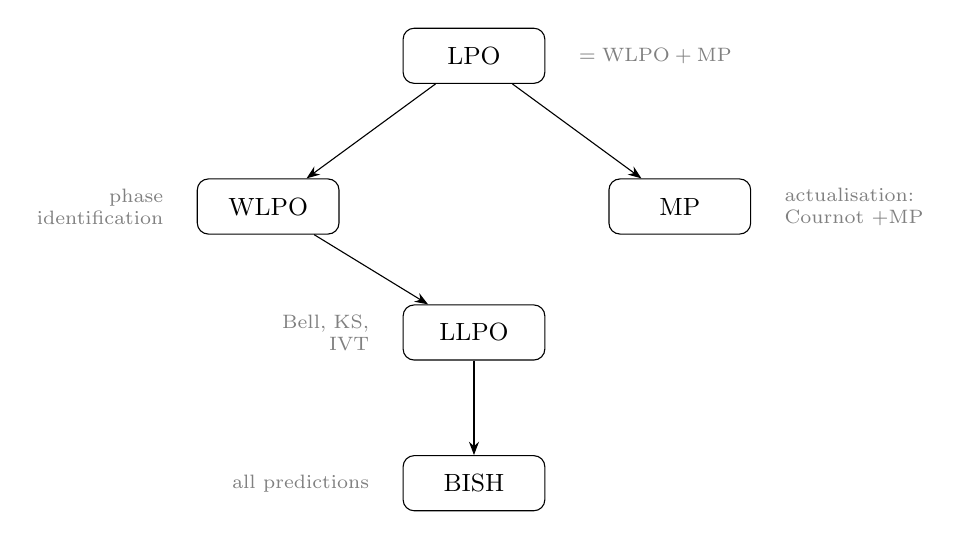
\begin{tikzpicture}[
  node distance=1.4cm,
  every node/.style={font=\small},
  principle/.style={draw,rounded corners,minimum width=1.8cm,
                    minimum height=0.7cm,align=center},
]
  \node[principle] (lpo) {$\LPO$};
  \node[principle, below left=1.2cm and 0.8cm of lpo] (wlpo) {$\WLPO$};
  \node[principle, below right=1.2cm and 0.8cm of lpo] (mp) {$\MP$};
  \node[principle, below=2.8cm of lpo] (llpo) {$\LLPO$};
  \node[principle, below=1.2cm of llpo] (bish) {$\BISH$};

  \draw[-{Stealth}] (lpo) -- (wlpo);
  \draw[-{Stealth}] (lpo) -- (mp);
  \draw[-{Stealth}] (wlpo) -- (llpo);
  \draw[-{Stealth}] (llpo) -- (bish);

  \node[right=0.3cm of lpo, font=\scriptsize, text=gray]
    {$= \WLPO + \MP$};
  \node[left=0.3cm of wlpo, font=\scriptsize, text=gray,align=right]
    {phase\\identification};
  \node[right=0.3cm of mp, font=\scriptsize, text=gray,align=left]
    {actualisation:\\Cournot $+ \MP$};
  \node[left=0.3cm of llpo, font=\scriptsize, text=gray,align=right]
    {Bell, KS,\\IVT};
  \node[left=0.3cm of bish, font=\scriptsize, text=gray,align=right]
    {all predictions};
\end{tikzpicture}
\caption{The partial order of omniscience principles with physical
annotations.  $\WLPO$ and~$\MP$ are independent; their join
is~$\LPO$ (Ishihara, 2006).  $\FT$ and~$\DC$ are
independent of the entire chain and dispensable for
physics~\cite{Lee26P23}.}
\label{fig:hierarchy}
\end{figure}

Key relationships: $\WLPO + \MP = \LPO$
(Ishihara~\cite{Ishihara2006}).  $\WLPO$ and~$\MP$ are
independent---neither implies the other (model-theoretic
separation).  $\LLPO$ is independent of~$\MP$
(Bridges and Richman~\cite{BridgesRichman1987}).
The Fan Theorem is independent of all the above and enters
physics only as scaffolding (Paper~23).

\subsection{Consequence for the Ceiling}

The $\BISH + \LPO$ ceiling already contains~$\MP$.  Any physical
system whose calibration involves a thermodynamic limit---computed
via Fekete's Subadditive Lemma (Paper~29: Fekete $\equiv$
$\LPO$~\cite{Lee26P29})---automatically has~$\MP$ available.
No new tier is needed.  This corrects Paper~22's implicit framing
that~$\MP$ represented a cost beyond the existing ceiling.

Paper~23~\cite{Lee26P23} established that the Fan Theorem is
independent of~$\LPO$, $\MP$, and the entire omniscience chain.
The hierarchy therefore has four distinct roles in mathematical
physics: $\LPO$ (thermodynamic limits), $\WLPO$ (phase
identification), $\LLPO$ (quantum foundations), $\MP$
(actualisation), and~$\FT$ (scaffolding)---with $\FT$ and~$\DC$
dispensable.

% ====================================================================
\section{The BISH Content of Exponential Decay}
\label{sec:bish-decay}

\subsection{Theorem~2}

\begin{theorem}[Detection time is $\BISH$]
\label{thm:detection}
For all $\lambda > 0$ and $\varepsilon \in (0,1)$, there exists
a computable $t_0$ such that $\exp(-\lambda t_0) < \varepsilon$.
The witness is
\[
  t_0 = \frac{\log(1/\varepsilon) + 1}{\lambda}.
\]
\end{theorem}

\begin{proof}
\emph{Positivity:} Since $\varepsilon < 1$, we have
$1/\varepsilon > 1$, so $\log(1/\varepsilon) > 0$, hence
$\log(1/\varepsilon) + 1 > 0$, and $t_0 > 0$ (dividing by
$\lambda > 0$).
\emph{Bound:} $\lambda \cdot t_0 =
\log(1/\varepsilon) + 1 > \log(1/\varepsilon)$, so
$\exp(-\lambda t_0) < \exp(-\log(1/\varepsilon)) = \varepsilon$.
\end{proof}

This is~$\BISH$: an explicit formula, no limits, no search, no
omniscience.

\subsection{Correction of Paper~22}

Paper~22 proved that ``eventual decay for a rate~$\lambda$
known only to be nonzero'' is equivalent to~$\MP$.  This formal
equivalence is correct and is not retracted.  The binary-sequence
encoding (where $\lambda$ encodes a sequence with
$\lnot(\lambda = 0)$ but not $\lambda \mathrel{\#} 0$) makes
this a valid mathematical equivalence.

But the physical situation is different.  A measured decay rate
$\lambda_0$ is a known positive rational (with error bars).
For any such~$\lambda_0$, the detection time~$t_0$ is a
closed-form $\BISH$ witness.  The~$\MP$ content enters not
through computing the probability or the detection
time---both~$\BISH$---but through asserting that a specific atom
actually decays~(\S\ref{sec:cournot}).

\subsection{Significance}

Every computable quantity in exponential decay---the survival
probability, the detection time, the probability distribution,
the moments---is~$\BISH$.  No omniscience principle is needed
for the mathematics.  The distinction between mathematical
prediction ($\BISH$) and physical actualisation ($\MP$) is the
central structural finding of this paper.

% ====================================================================
\section{Cournot's Principle and Physical Actualisation}
\label{sec:cournot}

\subsection{The Postulate}

\begin{definition}[Cournot's Principle, 1843]
An event whose probability is zero does not occur in a single
realisation of the experiment.
\end{definition}

This is not a theorem.  It is a physical
postulate~\cite{Cournot1843}---the bridge between mathematical
probability and empirical physics.  Without Cournot's Principle,
probability theory describes ensembles and limiting frequencies.
It says nothing about what happens to a specific atom in a
specific experiment.  With Cournot's Principle, measure-zero
exclusions become physical impossibilities: if the set of eternal
survivors has probability zero, then this atom is not an eternal
survivor.

\subsection{The Three-Step Actualisation Chain}

For radioactive decay with rate $\lambda > 0$:
\begin{enumerate}[nosep]
\item \textbf{BISH:} $P(\text{survive forever}) =
  \lim_{t\to\infty} \exp(-\lambda t) = 0$.  Computable limit
  of a computable function.  The eternal survival set has measure
  zero.
\item \textbf{Cournot:} The actual atom's trajectory does not
  belong to the measure-zero eternal survival set.  Therefore:
  $\lnot(\forall t,\;\text{undecayed at } t)$.
\item \textbf{MP:} From
  $\lnot(\forall t,\;\text{undecayed at } t)$, extract
  $\exists t,\;\text{decayed by } t$.
\end{enumerate}
Step~1 is mathematics.  Step~2 is a physical postulate.
Step~3 is Markov's Principle.  The chain is:
$\BISH \to \text{Cournot} \to \lnot\forall \to \MP \to \exists$.

\subsection{What Each School Says}

\textbf{Brouwer} accepts step~1.  Rejects step~3---the
$\lnot\forall \to \exists$ inference is illegitimate without a
bounded construction.  Also suspicious of step~2 as a mathematical
principle (Cournot is physics, not mathematics).  Conclusion:
mathematics can compute all probabilities but cannot assert
actual decay.

\textbf{Markov} accepts all three steps.  Step~3 is exactly~$\MP$,
which the Russian school endorses.  The atom decays because a
process that cannot fail to terminate does terminate.  Conclusion:
actual decay is a legitimate mathematical consequence.

\textbf{Bishop} accepts step~1.  Takes no position on steps~2--3.
$\BISH$ computes the probabilities.  Whether you additionally
assert actual decay is outside~$\BISH$'s scope.  Conclusion:
the mathematical content is constructive; the rest is your problem.

This is not an academic disagreement.  It concerns whether
mathematical physics can assert that unstable things actually fall
apart.  The three most influential schools of constructive
mathematics give three different answers to the most basic
physical process imaginable.

% ====================================================================
\section{Poincar\'{e} Recurrence and False Vacuum Decay}
\label{sec:calibrations}

\subsection{Poincar\'{e} Recurrence: BISH Content}

\begin{theorem}[Non-return set has measure zero]
\label{thm:poincare}
Let $\varphi$ be a measure-preserving map on a finite measure
space $(X,\mu)$.  For any measurable set~$A$, let
$B = \{x \in A : \forall k \ge 1,\;\varphi^k(x) \notin A\}$.
Then $\mu(B) = 0$.
\end{theorem}

\begin{proof}[Proof sketch]
The preimages $\varphi^{-n}(B)$ are pairwise disjoint
(combinatorial, $\BISH$) and equimeasured (measure preservation,
$\BISH$).  If $\mu(B) > 0$, their union has infinite measure,
contradicting $\mu(X) < \infty$.  So $\mu(B) = 0$.
$\BISH$ throughout.
\end{proof}

The \Lean{} formalization wraps \Mathlib{}'s
\texttt{Conservative.measure\_mem\_forall\_ge\_image\_notMem\_eq\_zero}.

\subsection{Poincar\'{e} Recurrence: MP Content}

``This specific orbit returns to~$A$'' requires Cournot
($\omega \notin B$ since $\mu(B)=0$) followed
by~$\MP$ ($\lnot\forall\lnot \to \exists$).  The logical
structure is identical to radioactive decay.

\textbf{Notable difference.}\quad
Unlike radioactive decay, Poincar\'{e} recurrence has no
computable return time.  \Cref{thm:detection} gives an explicit
$\BISH$ detection time for decay.  The return time for
Poincar\'{e} recurrence depends on Diophantine properties of
the orbit and is generally not computable.  Yet the logical
cost is the same: Cournot $+ \MP$.  The non-computability of
the return time adds nothing to the logical cost.  The
obstacle is witness quality (no bound available), not the
principle needed (still~$\MP$).

\subsection{False Vacuum Decay}

The false vacuum tunnelling rate $\Gamma/V$ is computable from
the bounce action via Picard iteration ($\BISH$).  The survival
probability $P(T) = \exp(-(\Gamma/V)\cdot V \cdot T)$ is
computable for all finite~$T$.  The detection time is computable.
The probability of eternal metastability is zero.

The actualisation assertion---``the false vacuum eventually
decays somewhere''---is Cournot $+ \MP$.  Structurally identical
to radioactive decay.  In the \Lean{} formalization,
\texttt{vacuum\_decays\_mp} is defined as
\texttt{atom\_decays\_mp} with the tunnelling rate in place of
the decay rate.

\subsection{The Pattern}

\begin{table}[ht]
\centering
\begin{tabular}{lcc}
\toprule
\textbf{System} & \textbf{Math.\ prediction} &
  \textbf{Physical actualisation} \\
\midrule
Radioactive decay & $\BISH$ (detection time) & Cournot $+ \MP$ \\
Poincar\'{e} recurrence & $\BISH$ ($\mu = 0$) & Cournot $+ \MP$ \\
False vacuum decay & $\BISH$ (detection time) & Cournot $+ \MP$ \\
\bottomrule
\end{tabular}
\caption{Three physically distinct systems, one logical mechanism,
the same axiom cost.}
\label{tab:calibrations}
\end{table}

% ====================================================================
\section{Three Readings of the Calibration Table}
\label{sec:readings}

\subsection{The Strict Bishopian Reading}

Physics = computable predictions only.  Every quantity an
experiment can check to finite precision is~$\BISH$.  $\LPO$
enters through the thermodynamic limit, which is a mathematical
idealisation---no experiment measures an infinite system.
Under this reading, the logical constitution of measured physics
is \textbf{BISH alone}.  $\LPO$ is the cost of a useful
idealisation.  $\MP$ is irrelevant.

This reading is defensible but radical.  It says phase transitions
do not ``really'' happen---there is no sharp Curie temperature,
just a very steep crossover.  Many physicists would object.
But the objection is physical, not logical.

\subsection{The Standard Reading (Paper~40)}

Physics = computable predictions + thermodynamic limits.  The
infinite-volume limit is part of physics because physicists use
it, its predictions are confirmed, and the alternative (working
only with finite systems) is computationally intractable.  $\LPO$
is genuinely required.  Under this reading, the logical
constitution is $\mathbf{\BISH + \LPO}$.  $\MP$ is subsumed
(since $\LPO \Rightarrow \MP$).

This is Paper~40's position and the programme's default reading.

\subsection{The Inclusive Reading}

Physics = computable predictions + thermodynamic limits + physical
actualisation.  The assertion ``this atom decays'' is an empirical
prediction, confirmed trillions of times.  Cournot's Principle is
a physical commitment.  $\MP$ is part of the logical constitution.
Under this reading: $\mathbf{\BISH + \LPO + \MP}$.
But $\LPO \Rightarrow \MP$, so this reduces to
$\mathbf{\BISH + \LPO}$.
The~$\MP$ content is present but not independent---automatically
subsidized by the thermodynamic limit.

This reading adds nothing to the ceiling but makes explicit that
actualisation is a distinct physical commitment with a distinct
logical signature.

\subsection{What the Programme Contributes}

The programme does not choose between these readings.  It provides
the measurements that make the choice precise.  Before the
programme, ``how much non-constructive reasoning does physics
need?''\ was a vague philosophical question.  After the programme,
it is a question with three precise answers---$\BISH$,
$\BISH + \LPO$, or $\BISH + \LPO + \MP$---corresponding to three
precise demarcation choices.  The measurements are the same
regardless of which reading you adopt.  This is the paper's
central contribution: the meta-mathematical precision of the
question, not the answer.

% ====================================================================
\section{The Fine Structure of the Ceiling}
\label{sec:fine}

\subsection{Three Universal Mechanisms}

\begin{table}[ht]
\centering
\begin{tabular}{lll}
\toprule
\textbf{Principle} & \textbf{Mechanism} & \textbf{Physical context} \\
\midrule
$\LPO$  & Fekete's Subadditive Lemma & Finite $\to$ infinite volume \\
$\LLPO$ & Intermediate Value Theorem  & Root-finding, measurement \\
$\MP$   & Cournot $+ \lnot\forall \to \exists$
         & Probability $\to$ actuality \\
\bottomrule
\end{tabular}
\caption{Each principle enters physics through a single mechanism
across all calibrations examined.}
\label{tab:mechanisms}
\end{table}

\subsection{Nature at the Disputed Border}

Of all principles in the constructive hierarchy, $\MP$ is the one
the three schools disagree about.  And~$\MP$ governs the most
basic physical process imaginable: a single unstable thing
decaying.  Not a phase transition ($\LPO$).  Not a quantum
foundation result ($\LLPO$).  Not a compactness argument ($\FT$).
Just: a thing falls apart, eventually.

The programme cannot determine whether this is a deep fact or a
coincidence.  But it can state precisely what the coincidence is:
the physical process of stochastic actualisation---the passage
from ``probability says this will happen'' to ``it actually
happens''---sits at exactly the principle where the constructive
schools part company.
The structure of the~$\MP$ step---from $\lnot\forall$ to
$\exists$ for outcomes of a random process---is identical to a
well-studied phenomenon in constructive probability theory.
A Martin-L\"{o}f random binary sequence cannot be identically
zero ($\BISH$, since $\{000\ldots\}$ has measure zero).
But asserting that a specific random sequence has a~1 somewhere
requires~$\MP$.
The literature on constructive measure theory
(Bishop~\cite{Bishop1967}; Spitters; Chan) has explored this
boundary from the mathematical side.  The programme adds the
physical side.

% ====================================================================
\section{Relation to the Programme}
\label{sec:programme}

\subsection{Paper~22 (Markov Decay)}

Paper~22 established the formal equivalence between eventual decay
(binary-sequence encoding) and~$\MP$.  Paper~43 corrects the
framing: the mathematical prediction is~$\BISH$; $\MP$ enters
only through physical actualisation.  Paper~22's formal results
are correct and not retracted.  Six interpretive edits are
specified in the proof document.
The $\LPO \Rightarrow \MP$ proof was always implicit in the
hierarchy but not previously stated in the programme.

\subsection{Paper~23 (Fan Theorem)}

Paper~23~\cite{Lee26P23} established that the Fan Theorem is
equivalent to CompactOptimization and independent of~$\LPO$,
$\MP$, $\WLPO$, and~$\LLPO$.
Paper~43 completes the logical map: the four distinct roles in
mathematical physics are~$\LPO$ (thermodynamic limits), $\LLPO$
(quantum foundations), $\MP$ (actualisation), and~$\FT$
(scaffolding).  Of these, $\FT$ and~$\DC$ are dispensable.
The three indispensable principles---$\LPO$, $\LLPO$,
$\MP$---sit in a single partial order with~$\LPO$ at the top.

\subsection{Paper~40 (The Ceiling)}

Paper~40~\cite{Lee26P40} declared $\BISH + \LPO$ as the ceiling.
Paper~43 does not change this verdict.
The three readings of the calibration table (\S\ref{sec:readings})
show that Paper~40's position is one of three defensible
choices---but all three yield the same formal ceiling
($\BISH + \LPO$), since~$\MP$ is subsumed.

\subsection{Paper~29 (Fekete/LPO)}

Paper~29~\cite{Lee26P29} established that Fekete's Subadditive
Lemma is equivalent to~$\LPO$.  Since $\LPO \Rightarrow \MP$,
every system calibrated at~$\LPO$ via Fekete automatically
has~$\MP$ available.  The actualisation cost is always subsidized
by the thermodynamic limit cost.  This is why the ceiling does
not extend.

% ====================================================================
\section{Lean~4 Formalization}
\label{sec:lean}

\subsection{Code Architecture}

\begin{verbatim}
P43_Actualisation/
  Defs/         Principles.lean, Cournot.lean, Decay.lean
  Hierarchy/    LPOImpliesMP.lean
  BISHContent/  ExponentialWitness.lean, PoincareMeasure.lean
  Actualisation/ RadioactiveDecay.lean, PoincarePointwise.lean,
                 FalseVacuum.lean
  Assembly/     FineStructure.lean, AxiomAudit.lean
  Main.lean
\end{verbatim}

Twelve source files, approximately~770 lines.  Builds with
\texttt{lake build} on \Lean{}~4.28.0 with \Mathlib{}.
Zero errors, zero \texttt{sorry}, zero warnings.

\medskip\noindent
\textbf{AI-assisted formalization methodology.}\quad
The \Lean{} code was developed with AI assistance (Claude,
Anthropic).  All proofs are machine-checked by the \Lean{}~4
type checker.  The AI assistant proposed proof strategies; the
type checker verified correctness.  No proof step relies on
AI judgment alone.

\subsection{Bridge Axioms}

Two custom axioms:
\begin{enumerate}[nosep]
\item \texttt{cournot}---Cournot's Principle, encoding the
  physical postulate that measure-zero events do not occur in
  single realisations.
\item \texttt{survival\_prob\_zero}---a bridge from the
  exponential probability model to the measure-space formulation.
\end{enumerate}
Markov's Principle appears as a \emph{hypothesis} in theorem
statements, not as an axiom---this is by design.  The programme
takes principles as hypotheses, allowing the formalization to
remain agnostic about which school is adopted.

\subsection{Code Vignette: The Actualisation Chain}

\begin{lstlisting}[caption={The three-step actualisation chain for
radioactive decay (\texttt{RadioactiveDecay.lean}).}]
theorem atom_decays_mp
    {O : Type*} [MeasurableSpace O] {u : Measure O}
    (hMP : MarkovPrinciple)
    (decayed : O -> N -> Bool)
    (undecayed : O -> N -> Prop)
    (h_equiv : forall w t, undecayed w t <-> decayed w t = false)
    (rate : R) (hr : 0 < rate)
    (h_model : forall t, u {w | undecayed w t} =
      ENNReal.ofReal (survivalProb rate t))
    (w : O) :
    exists t, decayed w t = true := by
  apply hMP (fun n => decayed w n)      -- Step 3: MP
  intro h_all_false
  apply not_eternal_survival undecayed rate hr h_model w
                                        -- Step 2: Cournot
  intro t
  rw [h_equiv]                          -- Step 1: BISH encoding
  exact h_all_false t
\end{lstlisting}

The three-step chain is visible in the proof term: $\MP$ is
applied first (outermost), then Cournot (via
\texttt{not\_eternal\_survival}), then the $\BISH$ encoding
(rewriting via \texttt{h\_equiv}).

\subsection{CRM Audit}

\begin{table}[ht]
\centering
\begin{tabular}{lll}
\toprule
\textbf{Module} & \textbf{Custom axioms} & \textbf{Infrastructure} \\
\midrule
Hierarchy ($\LPO \to \MP$, etc.) & None & \texttt{propext} \\
$\BISH$ content (Thms.~2, 3) & None
  & \texttt{propext}, \texttt{Classical.choice} \\
Actualisation (decay, rec., vac.) & \texttt{cournot},
  \texttt{survival\_prob\_zero}
  & \texttt{propext}, \texttt{Classical.choice} \\
Assembly (fine structure) & None
  & \texttt{propext}, \texttt{Classical.choice} \\
\bottomrule
\end{tabular}
\caption{CRM axiom audit summary.
\texttt{Classical.choice} and \texttt{Quot.sound} appear through
\Mathlib{}'s real number infrastructure (Cauchy completion), not
through proof content.  Constructive stratification is established
by proof content, not by axiom checker output
(Paper~10, \S Methodology).}
\label{tab:audit}
\end{table}

% ====================================================================
\section{Reproducibility}
\label{sec:repro}

The complete \Lean{}~4 formalization is archived at
\textbf{doi:10.5281/zenodo.18665418}.

\begin{itemize}[nosep]
\item \textbf{Toolchain:} \texttt{leanprover/lean4:v4.28.0}.
\item \textbf{Dependency:} \Mathlib{} (pinned via
  \texttt{lake-manifest.json}).
\item \textbf{Build:}
  \texttt{cd P43\_Actualisation \&\& lake exe cache get
  \&\& lake build}.
\item \textbf{Result:} 0~errors, 0~\texttt{sorry}, 0~warnings.
  Twelve source files, ${\sim}770$~lines.
\item All theorems verified by the \Lean{}~4 type checker.
  The axiom audit (\texttt{Assembly/AxiomAudit.lean}) confirms
  that $\BISH$ theorems use only \Mathlib{} infrastructure,
  hierarchy theorems use \texttt{propext} only, and actualisation
  theorems add exactly the two declared bridge axioms.
\end{itemize}

% ====================================================================
\begin{thebibliography}{99}

\bibitem{Bishop1967}
E.~Bishop,
\emph{Foundations of Constructive Analysis},
McGraw-Hill (1967).

\bibitem{BridgesRichman1987}
D.~Bridges and F.~Richman,
\emph{Varieties of Constructive Mathematics},
Cambridge University Press (1987).

\bibitem{BridgesVita2006}
D.~Bridges and L.~Vita,
\emph{Techniques of Constructive Analysis},
Springer (2006).

\bibitem{Markov1954}
A.~A.~Markov,
\emph{Theory of Algorithms},
Trudy Mat.\ Inst.\ Steklov \textbf{42} (1954).

\bibitem{Cournot1843}
A.~A.~Cournot,
\emph{Exposition de la Th\'{e}orie des Chances et des
Probabilit\'{e}s},
Hachette (1843).

\bibitem{Ishihara2006}
H.~Ishihara,
``Constructive reverse mathematics: compactness properties,''
in \emph{From Sets and Types to Topology and Analysis},
Oxford Logic Guides~48, Oxford University Press (2005),
pp.~245--267.

\bibitem{ShaferVovk2001}
G.~Shafer and V.~Vovk,
\emph{Probability and Finance: It's Only a Game!},
Wiley (2001).

\bibitem{Lee26P10}
P.~C.-K.~Lee,
``Paper~10: Calibration table and methodology,''
CRM Programme (2026).

\bibitem{Lee26P23}
P.~C.-K.~Lee,
``Paper~23: The Fan Theorem and the constructive cost
of optimization,''
CRM Programme (2026).

\bibitem{Lee26P29}
P.~C.-K.~Lee,
``Paper~29: Fekete's Subadditive Lemma is equivalent to LPO,''
CRM Programme (2026).
doi:10.5281/zenodo.18632776.

\bibitem{Lee26P40}
P.~C.-K.~Lee,
``Paper~40: Defending the BISH+LPO ceiling,''
CRM Programme (2026).
doi:10.5281/zenodo.18654773.

\bibitem{Lee26P41}
P.~C.-K.~Lee,
``Paper~41: Axiom calibration of the AdS/CFT correspondence,''
CRM Programme (2026).
doi:10.5281/zenodo.18654780.

\bibitem{Lee26P42}
P.~C.-K.~Lee,
``Paper~42: Axiom calibration of the cosmological constant problem,''
CRM Programme (2026).
doi:10.5281/zenodo.18654789.

\bibitem{BrattkaEtAl2012}
V.~Brattka, G.~Gherardi, and A.~Marcone,
``The Bolzano--Weierstrass theorem is the jump of weak
K\H{o}nig's lemma,''
\emph{Annals of Pure and Applied Logic}
\textbf{163}(6), 623--655 (2012).

\bibitem{Fekete1923}
M.~Fekete,
``\"{U}ber die Verteilung der Wurzeln bei gewissen
algebraischen Gleichungen mit ganzzahligen Koeffizienten,''
\emph{Mathematische Zeitschrift} \textbf{17}, 228--249 (1923).

\end{thebibliography}

\end{document}

